\section{Reliable 1Pipe}
\label{sec:reliable}

Now, we design reliable \sys{} that handles packet loss and failure.
When a receiver delivers a message with timestamp $T$, it must make sure that all messages below $T$ are delivered.
So, if a receiver is unaware of packet loss, it cannot reliably deliver messages according to the barrier timestamp.
Even if the switch is capable of detecting lost packets, there is still a problem. %because \emph{host failure and packet loss may happen together}.
For example, host $A$ sends to $B$, then sends to $C$ via a different path. The packet $A \rightarrow B$ is lost on the way. Then, $A$ crashes. The packet $A \rightarrow C$ is delivered, while $A \rightarrow B$ cannot be recovered. Failure to deliver $A \rightarrow B$ and delivery of $A \rightarrow C$ violates reliable ordering property.
Although the probability of simultaneous packet loss and host failure is very low, reliable \sys{} still needs to take this into account.


\begin{figure}[t]
\centering
	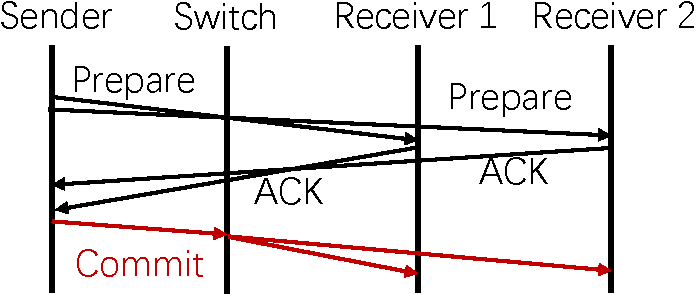
\includegraphics[width=.3\textwidth]{images/2PC.pdf}
	\caption{Two Phase Commit in reliable \sys{}.}
	\label{fig:2PC}
\end{figure}

\begin{figure}[t]
	\centering
	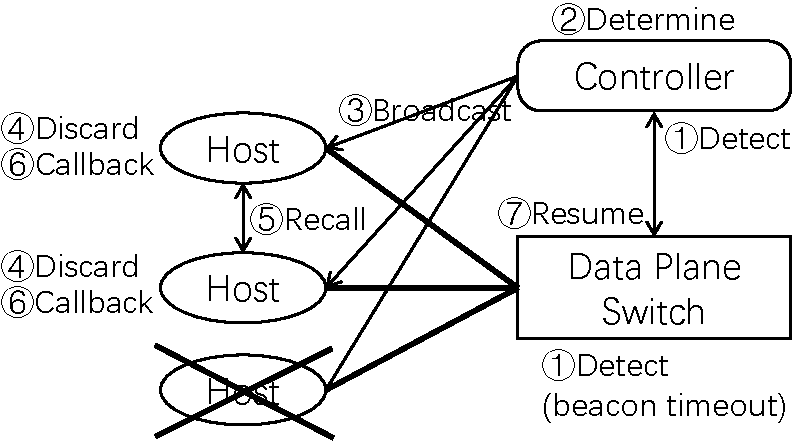
\includegraphics[width=.35\textwidth]{images/failure_recovery.pdf}
	\caption{Failure recovery in reliable \sys{}.}
	\label{fig:failure_recovery}
\end{figure}

Our key idea is a \emph{Two Phase Commit (2PC)} approach:

\begin{ecompact}
\item \textbf{Prepare phase}: Sender puts messages into send buffer, and transmits them with timestamps. Network switches do NOT need to aggregate timestamp barriers. Receivers store the messages in receive buffer, and respond with ACKs. Senders wait for ACKs to detect packet loss, and retransmit messages if packets are lost in-flight.
\item \textbf{Commit phase}: When a sender collects all ACKs below or equal to $T$, it sends a \emph{commit message} that carries \emph{commit barrier} $T$. The commit message is sent to the neighbor switch rather than the receivers, as the red arrow in Figure~\ref{fig:2PC} shows. Each switch aggregates minimum commit barriers on input links, and produce commit barriers that propagate to output links. This timestamp aggregation procedure is exactly the same as Sec.\ref{sec:loss-free}. A receiver delivers messages below or equal to $T$ in receive buffer when it receives a commit barrier $T$.
\end{ecompact}



\parab{Failures of processes, hosts, switches, and links.}
Like in Sec.~\ref{sec:beacon}, crash failure of a component is detected by its neighbors not hearing any message after a timeout.
However, a failed component cannot be simply removed as in Sec.~\ref{sec:beacon}, because otherwise, the in-flight messages sent by the failed component cannot be consistently delivered or discarded.

To achieve restricted failure atomicity in Sec.\ref{subsec:abstration}, we use the network controller in data centers \revise{to detect failures via beacon timeout.}
The controller itself is replicated using Paxos~\cite{lamport1998part} or Raft~\cite{raft}, so, it is highly available, and only one controller is active at any time.
\revise{The controller needs to determine which processes fail and when they fail.
The former question is easier to answer. \emph{A process that disconnects from controller in routing graph is regarded as failed}. For example, if a host or the only network link from a host fails, all processes on it are disconnected from the data center network, so they are considered to fail simultaneously.	If a Top-of-Rack (ToR) switch fails, and hosts in the rack are only connected to one switch, then all processes in the rack are considered to fail.}

\revise{The latter question, when processes fail, is harder to answer. The challenge is that we cannot reliably determine the last committed and delivered timestamp of a process.
Because there is a propagation delay from committing a timestamp to delivering the timestamp to receivers, it is possible to find a timestamp $T$ committed by a failed process $P$ but not propagated to any receiver, so that all receivers have received messages from $P$ before $T$ in receive buffer (and hence can deliver them), but no messages after $T$ have been delivered, so they can be discarded.
\emph{Failure timestamp} of $P$ is defined as such, which is computed as the maximum last commit timestamp reported by all neighbors of $P$. If multiple failures occur simultaneously, we try to find a set of correct nodes in routing graph that separates failed nodes and all correct receivers.
If such a set cannot be found due to network partition, then we use a greedy algorithm to find a set to separate as many receivers as possible. The non-separable receivers sacrifice atomicity because some messages after $T$ may have been delivered.}


The procedure to handle failure is as follows \revise{and shown in Figure~\ref{fig:failure_recovery}}: (see Appendix for correctness analysis)

\begin{ecompact}
\item \textbf{Detect}: The neighbors of failed components notifies controller along with its last commit timestamp $T$.
\item \textbf{Determine}: Controller determines failed processes and their failure timestamps according to the routing graph.
\item \textbf{Broadcast}: Controller broadcasts the failed processes $P$ and its failure timestamp $T$ to all correct processes.
\item \textbf{Discard}: Each correct process discards messages sent from $P$ with timestamp higher than $T$ in receive buffer.
\item \textbf{Recall}: Each correct process discards messages sent to $P$ in send buffer, which are waiting for ACK from $P$. If a discarded message is in a scattering, according to failure atomicity, the scattering needs to be aborted, \emph{i.e.}, messages to other receivers \emph{in the same scattering} need to be recalled. The sender sends a \emph{recall} message to such receivers, then each of the receivers discards the messages in receive buffer and responds ACK to the sender. The sender completes Recall after collecting the ACKs.
\item \textbf{Callback}: Each correct process executes the process failure callback registered in Table~\ref{tab:abstraction}, which enables applications to customize failure handling. Then, it responds controller with a completion message.
\item \textbf{Resume}: Controller collects completions from all correct processes, and then notifies network components to remove input link from the failed component, thereby resuming barrier propagation.
%After all failed processes have been handled by all correct processes,
%Before this step, commit barrier $T$ from $P$ is never delivered.
\end{ecompact}

\parab{Controller Forwarding.} If a network failure affects connectivity between $S$ and $R$, the Commit phase in 2PC and the Recall step in failure handling may stall because $S$ repeatedly retransmits a message but cannot receive ACK from $R$.
In this case, $S$ asks controller to forward the message to $R$, and waits for ACK from controller. If controller also cannot deliver the message, $R$ will be announced as failed, and the undeliverable recall message is recorded. If controller receives ACK of a recall message but cannot forward it to $S$, $S$ will be announced as failed. In summary, if a process does not respond controller within timeout, it is considered as failed.

\parab{Receiver Recovery.} If a process recovers from failure,  \revise{\emph{e.g.}, the network link or switch recovers},
the process needs to consistently deliver or discard messages in receive buffer. The controller notifies process of its own failure. Then, the process contacts controller to get host failure notifications since its failure and undeliverable recall messages. \revise{After delivering buffered messages, the recovered process needs to join \sys{} as a new process. This is because if a process can fail and recover multiple times, the controller would need to record all failure and recovery timestamps, adding complexity.}

\parab{\revise{Limitations.}} \revise{If a process fails permanently, the last timestamp it has delivered cannot be known exactly, so, \sys{} only ensures all correct receivers and recovered receivers deliver messages consistently. In addition, when network partition occurs, separated receivers may deliver messages after failure timestamp. \sys{} relies on the application to coordinate such failures.}
%We expect future work to improve failure handling and atomicity.

%The 2PC procedure ensures that if a message $M$ from $S$ to $R$ with timestamp $T$ is delivered, then all messages from $S$ and below $T$ have been buffered in their corresponding receivers. If the receiver $R$ is correct when it receives commit barrier $T$, $M$ should be delivered.
%In addition, timestamp aggregation ensures that if a message to $R$ with $T$ is committed, all messages to $R$ below $T$ are also committed.

%The Discard step of failure handling ensures that a message $M: S \rightarrow R$ with timestamp $T$ is not delivered if $S$ fails before $T$. The Recall step ensures that if $M: S \rightarrow R$ and $M': S \rightarrow R'$ are in the same batch, $M$ is not delivered if $R'$ fails before $T$.

%Although the failure recovery process requires the controller to broadcast to all correct processes, it is only invoked when failure occurs, so, the overhead is limited.


%Consider crash failure only. No Byzantine failure. Controller is a perfect failure detector: every faulty process is eventually permanently suspected by every non-faulty process. Non-faulty process are never suspected. Controller itself is replicated using traditional Paxos / Raft.

%only guarantees reliable delivery in absence of host failure during packet loss recovery. Because packet loss is rare and host failure is infrequent, combined probability is very low. When host fail, cannot recover lost packets, but other packets may have delivered.